\subsection{Buca di potenziale a pareti infinite}
\[
\mathcal{H} = \frac{\hat{p}^2}{2m} + V(x), \quad V(x) = \left\{ \begin{matrix*}[l]
0 & |x| < a \\
V_0 \to +\infty & |x| > a
\end{matrix*} \right.
\]

La particella è intrappolata nella buca indipendentemente dall'energia che può avere e non supera la barriera (questa è la teoria classica).

Voglio sapere lo spettro di autostati di \( \mathcal{H} \) nella base delle coordinate. Allora:
\[
\mathcal{H} \ket{\psi_E} = E \ket{\psi_E}
\]
dove so \( \braket{x|\psi_E} = \psi_E(x) \).

Per \( |x| < a \)
\[
\braket{x|\mathcal{H}|\psi_E} = - \frac{\hbar^2}{2m} \frac{d^2}{dx^2} \psi_E(x) = E \psi_E(x).
\]

Per \( |x| > a \)
\[
\braket{x|\mathcal{H}|\psi_E} = - \frac{\hbar^2}{2m} \frac{d^2}{dx^2} \psi_E(x) = (E - V_0) \psi_E(x).
\]
\[
V_0 \to +\infty \Rightarrow \frac{d^2}{dx^2} \psi_E(x) = -\frac{2m}{\hbar^2} (E - V_0) \psi_E(x) \to +\infty, \forall E \Rightarrow \psi_E(x) = 0.
\]
Infatti fuori dalla buca una soluzione dell'equazione differenziale (con normalizzazione) è
\[
\psi_E(x) = N_E \exp \left\{ \pm \sqrt{\frac{2m}{\hbar^2}(V_0 - E)} x \right\}, \quad |x| > a.
\]
Deve restare valida la condizione
\[
\int_{-\infty}^{+\infty} |\psi(x)|^2 \, dx < +\infty
\]
quindi
\[
\psi_E(x) = N_E \exp \left\{ -\sqrt{\frac{2m}{\hbar^2}(V_0 - E)} x \right\} \quad (x > a),
\]
\[
\psi_E(x) = N_E \exp \left\{ \sqrt{\frac{2m}{\hbar^2}(V_0 - E)} x \right\} \quad (x < -a)
\]
Allora in generale ponendo \( k = \sqrt{\frac{2m}{\hbar^2}(V_0 - E)} \),
\[
\psi_E(x) = N_E e^{-k |x|} \quad (x > a)
\]
che per \( V_0 \to +\infty \) dà \( \psi_E \to 0 \). Questo impone come condizioni al contorno \( \psi_E(\pm a) = 0 \).

Per \( |x| < a \) invece
\[
\psi_E(x) = A_E' e^{ikx} + B_E' e^{-ikx}, \qquad E = \frac{\hbar^2 k^2}{2m}
\]
ovvero una combinazione lineare di seno e coseno
\[
\psi_E(x) = A_E \sin(kx) + B_E \cos(kx)
\]
e si presentano due casi.
\begin{enumerate}
\item \( B_E = 0 \Rightarrow \psi_E^I(x) = A_E \sin(kx) \) quindi per \( x = \pm a \) vale
\begin{align*}
\sin(ka) = -\sin(-ka) = 0 &\Rightarrow ka = \pi n \Rightarrow k_n = \frac{\pi}{a} n \Rightarrow \\
&\Rightarrow E_n = \frac{\hbar^2 \pi^2}{2m} \frac{n^2}{a^2}
\end{align*}
\item \( A_E = 0 \Rightarrow \psi_E^{II}(x) = B_E \cos(kx) \) e per \( x = \pm a \) ho
\begin{align*}
\cos(ka) = 0 \Rightarrow ka = (2n + 1) \frac{\pi}{2} &\Rightarrow k_n = \frac{\pi}{2a}(2n + 1) \Rightarrow \\ 
&\Rightarrow E_n = \frac{\hbar^2 \pi^2}{2m} \frac{(2n + 1)^2}{4a^2}
\end{align*}
\end{enumerate}

Quindi lo \textbf{spettro degli autovalori} è
\[
E_n = \frac{\hbar^2 k_n^2}{2m}, \qquad k_n = \frac{n\pi}{2a}
\]
e nel caso in cui \( n \) è pari ho la soluzione \( \psi_E^I \), mentre quando \( n \) è dispari ho la \( \psi_E^{II} \). Poiché infine \( L = 2a \) è la lunghezza della buca
\[
E_n = \frac{\hbar^2 n^2 \pi^2}{2 m L^2}.
\]
è anche possibile definire una \textbf{lunghezza d'onda} per le \( \psi_E \):
\[
\lambda_n = \frac{2\pi}{k_n} = \frac{2L}{n} \quad \Rightarrow \quad \frac{\lambda_n}{2} = \frac{L}{n}
\]
cioè la buca contiene \( n \) semilunghezze d'onda.

Definiamo allora lo \textbf{stato fondamentale} \( \psi^{II} \) come
\[
n = 1, \quad k = \frac{\pi}{2a}, \quad E = \frac{\hbar^2 \pi^2}{2 m L^2}
\]
e lo \textbf{stato eccitato} \( \psi^I \) per
\[
n = 2, \quad k = \frac{\pi}{a}, \quad E = \frac{2 \hbar^2 \pi^2}{m L^2}.
\]
Gli andamenti sono riportati in Figura \ref{buca_infinita}.
\begin{figure}
\centering
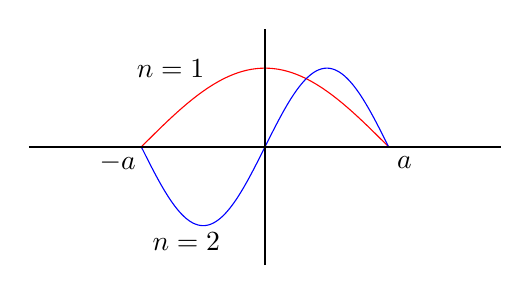
\begin{tikzpicture}
  \draw[color=red, domain=-pi/2:pi/2, samples=200, smooth] plot(\x,{cos(\x r)}) node[right] {};
  \node (A) at (-1.2,1) {\(n = 1\)};

  \draw[color=blue, domain=-pi/2:pi/2, samples=200, smooth] plot(\x,{sin(2*\x r)}) node[right] {};
  \node (B) at (-1,-1.2) {\(n = 2\)};

  \draw[thick] (-3,0) -- (3,0);
  \draw[thick] (0,-1.5) -- (0,1.5);

  \node (C) at (pi/2+.2,-.2) {\(a\)};
  \node (D) at (-pi/2-.3,-.2) {\(-a\)};
\end{tikzpicture}
\caption{Andamento dello stato fondamentale (rosso) e del primo stato eccitato (blu) per la buca di potenziale a pareti infinite.}
\label{buca_infinita}
\end{figure}

Pensando alle soluzioni come azione dell'operatore parità sulla funzione d'onda si ha
\[
\braket{x|\mathcal{P}|\psi} = \braket{-x|\psi} \; \Rightarrow \; \mathcal{P} \ket{\psi_E} = \begin{cases}
+ \ket{\psi_E} \text{ se ho } \psi^{II} \\
- \ket{\psi_E} \text{ se ho } \psi^I 
\end{cases}
\]
Inoltre \([\mathcal{H}, \mathcal{P}] = 0\), ed essendo \( \mathcal{P}^{-1} \mathcal{H} \mathcal{P} = \mathcal{H} \), le autofunzioni \( \psi_E \) sono gli autostati di \( \mathcal{H} \) e di \( \mathcal{P} \).

Era possibile dedurre lo stato ad energia minima dal principio di indeterminazione perché 
\[
\begin{cases}
\Delta x \leq L \Rightarrow \Delta^2 x \leq L^2 \\
\Delta^2 \hat{p} \Delta^2 \hat{x} \geq \frac{\hbar^2}{4}
\end{cases} \; \Rightarrow \; \Delta^2 \hat{p} \geq \frac{\hbar^2}{4L^2}
\]
avendo che l'impulso ha un valore minimo. Dunque non posso che avere un'energia minima.